%%%%%%%%%%%%%%%%%%%%%%%%%%%%%%%%%%%%%%%%%%%%%%%%%%%%%%%%%%%%%%%%%%%%%%%%%%
%
% 	Template for seminar reports
%
%%%%%%%%%%%%%%%%%%%%%%%%%%%%%%%%%%%%%%%%%%%%%%%%%%%%%%%%%%%%%%%%%%%%%%%%%%

%%%%%%%%%%%%%%%%%%%%%%%%%%%%%%%%%%%%%%%%%%%%%%%%%%%%%%%%%%%%%%%%%%%%%%%%%%
% 	Include layout and macros
%%%%%%%%%%%%%%%%%%%%%%%%%%%%%%%%%%%%%%%%%%%%%%%%%%%%%%%%%%%%%%%%%%%%%%%%%%

%% This LaTeX template is based on the following example file included in the ieeetran
%% package:
%% bare_conf.tex
%% V1.2
%% 2002/11/18
%% by Michael Shell
%% mshell@ece.gatech.edu
%% (requires IEEEtran.cls version 1.6b or later) with an IEEE conference paper.


% Note that the a4paper option is mainly intended so that authors in
% countries using A4 can easily print to A4 and see how their papers will
% look in print. Authors are encouraged to use U.S. letter paper when
% submitting to IEEE. Use the testflow package mentioned above to verify
% correct handling of both paper sizes by the author's LaTeX system.
%
% Also note that the "draftcls" or "draftclsnofoot", not "draft", option
% should be used if it is desired that the figures are to be displayed in
% draft mode.
%
% This paper can be formatted using the peerreviewca
% (instead of conference) mode.
\documentclass[conference, a4paper]{template/IEEEtran-modified}
% If the IEEEtran.cls has not been installed into the LaTeX system files,
% manually specify the path to it:
% \documentclass[conference]{../sty/IEEEtran}

\IEEEoverridecommandlockouts

% some very useful LaTeX packages include:

\usepackage{cite}       % Written by Donald Arseneau
                        % V1.6 and later of IEEEtran pre-defines the format
                        % of the cite.sty package \cite{} output to follow
                        % that of IEEE. Loading the cite package will
                        % result in citation numbers being automatically
                        % sorted and properly "ranged". i.e.,
                        % [1], [9], [2], [7], [5], [6]
                        % (without using cite.sty)
                        % will become:
                        % [1], [2], [5]--[7], [9] (using cite.sty)
                        % cite.sty's \cite will automatically add leading
                        % space, if needed. Use cite.sty's noadjust option
                        % (cite.sty V3.8 and later) if you want to turn this
                        % off. cite.sty is already installed on most LaTeX
                        % systems. The latest version can be obtained at:
                        % http://www.ctan.org/tex-archive/macros/latex/contrib/supported/cite/

%\usepackage{graphicx}  % Written by David Carlisle and Sebastian Rahtz
                        % Required if you want graphics, photos, etc.
                        % graphicx.sty is already installed on most LaTeX
                        % systems. The latest version and documentation can
                        % be obtained at:
                        % http://www.ctan.org/tex-archive/macros/latex/required/graphics/
                        % Another good source of documentation is "Using
                        % Imported Graphics in LaTeX2e" by Keith Reckdahl
                        % which can be found as esplatex.ps and epslatex.pdf
                        % at: http://www.ctan.org/tex-archive/info/
% NOTE: for dual use with latex and pdflatex, instead load graphicx like:
\ifx\pdfoutput\undefined
	\usepackage{graphicx}
\else
	\usepackage[pdftex]{graphicx}
\fi

% However, be warned that pdflatex will require graphics to be in PDF
% (not EPS) format and will preclude the use of PostScript based LaTeX
% packages such as psfrag.sty and pstricks.sty. IEEE conferences typically
% allow PDF graphics (and hence pdfLaTeX). However, IEEE journals do not
% (yet) allow image formats other than EPS or TIFF. Therefore, authors of
% journal papers should use traditional LaTeX with EPS graphics.
%
% The path(s) to the graphics files can also be declared: e.g.,
% \graphicspath{{../eps/}{../ps/}}
% if the graphics files are not located in the same directory as the
% .tex file. This can be done in each branch of the conditional above
% (after graphicx is loaded) to handle the EPS and PDF cases separately.
% In this way, full path information will not have to be specified in
% each \includegraphics command.
%
% Note that, when switching from latex to pdflatex and vice-versa, the new
% compiler will have to be run twice to clear some warnings.
\graphicspath{{figures/}}


%\usepackage{psfrag}    % Written by Craig Barratt, Michael C. Grant,
                        % and David Carlisle
                        % This package allows you to substitute LaTeX
                        % commands for text in imported EPS graphic files.
                        % In this way, LaTeX symbols can be placed into
                        % graphics that have been generated by other
                        % applications. You must use latex->dvips->ps2pdf
                        % workflow (not direct pdf output from pdflatex) if
                        % you wish to use this capability because it works
                        % via some PostScript tricks. Alternatively, the
                        % graphics could be processed as separate files via
                        % psfrag and dvips, then converted to PDF for
                        % inclusion in the main file which uses pdflatex.
                        % Docs are in "The PSfrag System" by Michael C. Grant
                        % and David Carlisle. There is also some information
                        % about using psfrag in "Using Imported Graphics in
                        % LaTeX2e" by Keith Reckdahl which documents the
                        % graphicx package (see above). The psfrag package
                        % and documentation can be obtained at:
                        % http://www.ctan.org/tex-archive/macros/latex/contrib/supported/psfrag/

%\usepackage{subfigure} % Written by Steven Douglas Cochran
                        % This package makes it easy to put subfigures
                        % in your figures. i.e., "figure 1a and 1b"
                        % Docs are in "Using Imported Graphics in LaTeX2e"
                        % by Keith Reckdahl which also documents the graphicx
                        % package (see above). subfigure.sty is already
                        % installed on most LaTeX systems. The latest version
                        % and documentation can be obtained at:
                        % http://www.ctan.org/tex-archive/macros/latex/contrib/supported/subfigure/

%\usepackage{url}       % Written by Donald Arseneau
                        % Provides better support for handling and breaking
                        % URLs. url.sty is already installed on most LaTeX
                        % systems. The latest version can be obtained at:
                        % http://www.ctan.org/tex-archive/macros/latex/contrib/other/misc/
                        % Read the url.sty source comments for usage information.

%\usepackage{stfloats}  % Written by Sigitas Tolusis
                        % Gives LaTeX2e the ability to do double column
                        % floats at the bottom of the page as well as the top.
                        % (e.g., "\begin{figure*}[!b]" is not normally
                        % possible in LaTeX2e). This is an invasive package
                        % which rewrites many portions of the LaTeX2e output
                        % routines. It may not work with other packages that
                        % modify the LaTeX2e output routine and/or with other
                        % versions of LaTeX. The latest version and
                        % documentation can be obtained at:
                        % http://www.ctan.org/tex-archive/macros/latex/contrib/supported/sttools/
                        % Documentation is contained in the stfloats.sty
                        % comments as well as in the presfull.pdf file.
                        % Do not use the stfloats baselinefloat ability as
                        % IEEE does not allow \baselineskip to stretch.
                        % Authors submitting work to the IEEE should note
                        % that IEEE rarely uses double column equations and
                        % that authors should try to avoid such use.
                        % Do not be tempted to use the cuted.sty or
                        % midfloat.sty package (by the same author) as IEEE
                        % does not format its papers in such ways.

\usepackage{amsmath}    % From the American Mathematical Society
                        % A popular package that provides many helpful commands
                        % for dealing with mathematics. Note that the AMSmath
                        % package sets \interdisplaylinepenalty to 10000 thus
                        % preventing page breaks from occurring within multiline
                        % equations. Use:
\interdisplaylinepenalty=2500
                        % after loading amsmath to restore such page breaks
                        % as IEEEtran.cls normally does. amsmath.sty is already
                        % installed on most LaTeX systems. The latest version
                        % and documentation can be obtained at:
                        % http://www.ctan.org/tex-archive/macros/latex/required/amslatex/math/



% Other popular packages for formatting tables and equations include:

%\usepackage{array}
% Frank Mittelbach's and David Carlisle's array.sty which improves the
% LaTeX2e array and tabular environments to provide better appearances and
% additional user controls. array.sty is already installed on most systems.
% The latest version and documentation can be obtained at:
% http://www.ctan.org/tex-archive/macros/latex/required/tools/

% Mark Wooding's extremely powerful MDW tools, especially mdwmath.sty and
% mdwtab.sty which are used to format equations and tables, respectively.
% The MDWtools set is already installed on most LaTeX systems. The lastest
% version and documentation is available at:
% http://www.ctan.org/tex-archive/macros/latex/contrib/supported/mdwtools/


% V1.6 of IEEEtran contains the IEEEeqnarray family of commands that can
% be used to generate multiline equations as well as matrices, tables, etc.


% Also of notable interest:

% Scott Pakin's eqparbox package for creating (automatically sized) equal
% width boxes. Available:
% http://www.ctan.org/tex-archive/macros/latex/contrib/supported/eqparbox/



% Notes on hyperref:
% IEEEtran.cls attempts to be compliant with the hyperref package, written
% by Heiko Oberdiek and Sebastian Rahtz, which provides hyperlinks within
% a document as well as an index for PDF files (produced via pdflatex).
% However, it is a tad difficult to properly interface LaTeX classes and
% packages with this (necessarily) complex and invasive package. It is
% recommended that hyperref not be used for work that is to be submitted
% to the IEEE. Users who wish to use hyperref *must* ensure that their
% hyperref version is 6.72u or later *and* IEEEtran.cls is version 1.6b
% or later. The latest version of hyperref can be obtained at:
%
% http://www.ctan.org/tex-archive/macros/latex/contrib/supported/hyperref/
%
% Also, be aware that cite.sty (as of version 3.9, 11/2001) and hyperref.sty
% (as of version 6.72t, 2002/07/25) do not work optimally together.
% To mediate the differences between these two packages, IEEEtran.cls, as
% of v1.6b, predefines a command that fools hyperref into thinking that
% the natbib package is being used - causing it not to modify the existing
% citation commands, and allowing cite.sty to operate as normal. However,
% as a result, citation numbers will not be hyperlinked. Another side effect
% of this approach is that the natbib.sty package will not properly load
% under IEEEtran.cls. However, current versions of natbib are not capable
% of compressing and sorting citation numbers in IEEE's style - so this
% should not be an issue. If, for some strange reason, the user wants to
% load natbib.sty under IEEEtran.cls, the following code must be placed
% before natbib.sty can be loaded:
%
% \makeatletter
% \let\NAT@parse\undefined
% \makeatother
%
% Hyperref should be loaded differently depending on whether pdflatex
% or traditional latex is being used:
%
%\ifx\pdfoutput\undefined
%\usepackage[hypertex]{hyperref}
%\else
%\usepackage[pdftex,hypertexnames=false]{hyperref}
%\fi
%
% Pdflatex produces superior hyperref results and is the recommended
% compiler for such use.



% *** Do not adjust lengths that control margins, column widths, etc. ***
% *** Do not use packages that alter fonts (such as pslatex).         ***
% There should be no need to do such things with IEEEtran.cls V1.6 and later.


%%%%%%%%%%%%%%%%%%%%%%%%%%%%%%%%%%%%%%%%%%%%%%%%%%%%%%%%%%%%%%%%%%%%%%%%%%
% 	Additional preamble
%%%%%%%%%%%%%%%%%%%%%%%%%%%%%%%%%%%%%%%%%%%%%%%%%%%%%%%%%%%%%%%%%%%%%%%%%%

% Additions to the IEEE preamble

\usepackage{tikz}

%%%%%%%%%%%%%%%%%%%%%%%%%%%%%%%%%%%%%%%%%%%%%%%%%%%%%%%%%%%%%%%%%%%%%%%%%%
% 	Page numbering (not on first page)
%%%%%%%%%%%%%%%%%%%%%%%%%%%%%%%%%%%%%%%%%%%%%%%%%%%%%%%%%%%%%%%%%%%%%%%%%%
\pagestyle{empty}

%%%%%%%%%%%%%%%%%%%%%%%%%%%%%%%%%%%%%%%%%%%%%%%%%%%%%%%%%%%%%%%%%%%%%%%%%%
% 	Correct bad hyphenation here
%%%%%%%%%%%%%%%%%%%%%%%%%%%%%%%%%%%%%%%%%%%%%%%%%%%%%%%%%%%%%%%%%%%%%%%%%%

\hyphenation{}

%%%%%%%%%%%%%%%%%%%%%%%%%%%%%%%%%%%%%%%%%%%%%%%%%%%%%%%%%%%%%%%%%%%%%%%%%%
% 	Enable support for German (for the title section)
%%%%%%%%%%%%%%%%%%%%%%%%%%%%%%%%%%%%%%%%%%%%%%%%%%%%%%%%%%%%%%%%%%%%%%%%%%

%
%%%%%%%%%%%%%%%%%%%%%%%%%%%%%%%%%%%%%%%%%%%%%%%%%%%%%%%%%%%%%%%%%%%%%%%%%%
% 	Anpassung an deutsche Texte
%%%%%%%%%%%%%%%%%%%%%%%%%%%%%%%%%%%%%%%%%%%%%%%%%%%%%%%%%%%%%%%%%%%%%%%%%%

\usepackage{ngerman}
\usepackage[latin1]{inputenc}   % f�r Umlaute 

\renewcommand{\abstractname}{Kurzfassung}      % statt Zusammenfassung, wie es ngerman definiert
\renewcommand{\keywordname}{Schl�sselworte}
%\renewcommand{\figurename}{Abb.}




%%%%%%%%%%%%%%%%%%%%%%%%%%%%%%%%%%%%%%%%%%%%%%%%%%%%%%%%%%%%%%%%%%%%%%%%%%
% 	Begin of the document
%%%%%%%%%%%%%%%%%%%%%%%%%%%%%%%%%%%%%%%%%%%%%%%%%%%%%%%%%%%%%%%%%%%%%%%%%%

\begin{document}

%%%%%%%%%%%%%%%%%%%%%%%%%%%%%%%%%%%%%%%%%%%%%%%%%%%%%%%%%%%%%%%%%%%%%%%%%%
% 	Paper title
%%%%%%%%%%%%%%%%%%%%%%%%%%%%%%%%%%%%%%%%%%%%%%%%%%%%%%%%%%%%%%%%%%%%%%%%%%

\title{A Tour of TensorFlow}

%%%%%%%%%%%%%%%%%%%%%%%%%%%%%%%%%%%%%%%%%%%%%%%%%%%%%%%%%%%%%%%%%%%%%%%%%%
% 	Author names and affiliations
%		-	multiple columns for up to three different affilitations are separated
%			by \and
%		- for over three affiliations, refer to ieeetran howto
%%%%%%%%%%%%%%%%%%%%%%%%%%%%%%%%%%%%%%%%%%%%%%%%%%%%%%%%%%%%%%%%%%%%%%%%%%

\author{
\authorblockN{Peter Goldsborough}
\authorblockA{Fakult\"{a}t f\"{u}r Informatik\\Technische Universit\"{a}t M\"{u}nchen\\
Email: peter.goldsborough@in.tum.de}
%\and
%\authorblockN{}
%\authorblockA{}
}

%%%%%%%%%%%%%%%%%%%%%%%%%%%%%%%%%%%%%%%%%%%%%%%%%%%%%%%%%%%%%%%%%%%%%%%%%%
% 	Special paper note (appears between title and authors)
%%%%%%%%%%%%%%%%%%%%%%%%%%%%%%%%%%%%%%%%%%%%%%%%%%%%%%%%%%%%%%%%%%%%%%%%%%

\specialpapernotice{Proseminar Data Mining}

%%%%%%%%%%%%%%%%%%%%%%%%%%%%%%%%%%%%%%%%%%%%%%%%%%%%%%%%%%%%%%%%%%%%%%%%%%
% 	Make title area
%%%%%%%%%%%%%%%%%%%%%%%%%%%%%%%%%%%%%%%%%%%%%%%%%%%%%%%%%%%%%%%%%%%%%%%%%%

\maketitle

%%%%%%%%%%%%%%%%%%%%%%%%%%%%%%%%%%%%%%%%%%%%%%%%%%%%%%%%%%%%%%%%%%%%%%%%%%
% 	For page number on first page
%%%%%%%%%%%%%%%%%%%%%%%%%%%%%%%%%%%%%%%%%%%%%%%%%%%%%%%%%%%%%%%%%%%%%%%%%%

%\thispagestyle{plain}

%%%%%%%%%%%%%%%%%%%%%%%%%%%%%%%%%%%%%%%%%%%%%%%%%%%%%%%%%%%%%%%%%%%%%%%%%%
% 	Abstract
%%%%%%%%%%%%%%%%%%%%%%%%%%%%%%%%%%%%%%%%%%%%%%%%%%%%%%%%%%%%%%%%%%%%%%%%%%

\begin{abstract}

  Deep learning is a branch of artificial intelligence employing deep neural
  network architectures that has significantly advanced the state-of-the-art in
  computer vision, speech recognition, natural language processing and other
  domains. In November 2015, Google released \emph{TensorFlow}, an open source
  deep learning software library for defining, training and deploying machine
  learning models. In this paper, we review TensorFlow and put it in context of
  modern deep learning concepts and software.We discuss its basic computational
  paradigms and distributed execution model, its programming interface as well
  as accompanying visualization toolkits. We then compare TensorFlow to
  alternative libraries such as Theano, Torch or Caffe on a qualitative as well
  as quantitative basis and finally comment on observed use-cases of TensorFlow
  in academia and industry.\vspace{0.5cm}
\end{abstract}

%%% Local Variables:
%%% mode: latex
%%% TeX-master: "../paper"
%%% End:


%%%%%%%%%%%%%%%%%%%%%%%%%%%%%%%%%%%%%%%%%%%%%%%%%%%%%%%%%%%%%%%%%%%%%%%%%%
% 	Keywords
%%%%%%%%%%%%%%%%%%%%%%%%%%%%%%%%%%%%%%%%%%%%%%%%%%%%%%%%%%%%%%%%%%%%%%%%%%

\begin{keywords}
  Artificial Intelligence, Machine Learning, Neural Networks, Distributed
  Computing, Open source software, Software packages
\end{keywords}


%%%%%%%%%%%%%%%%%%%%%%%%%%%%%%%%%%%%%%%%%%%%%%%%%%%%%%%%%%%%%%%%%%%%%%%%%%
% 	Sections, Subsections,...
%%%%%%%%%%%%%%%%%%%%%%%%%%%%%%%%%%%%%%%%%%%%%%%%%%%%%%%%%%%%%%%%%%%%%%%%%%

\section{Introduction}

Modern artificial-intelligence systems and machine-learning algorithms have
revolutionized approaches to a myriad of scientific and technological challenges
in a variety of fields. We can observe an immense proliferation in the quality
of state-of-the-art computer-vision and image-recognition, natural language
processing, speech recognition and other techniques. However, the major and most
obvious benefactor of this revolution is mankind itself. Personalized digital
assistants, recommendations on e-commerce platforms, financial fraud detection,
customized web-search results and social-network feeds as well as novel
breakthroughs in genomics have all been improved, if not enabled, by current
machine learning methods.

A particular branch of machine-learning, \emph{deep-learning}, has proven
especially effective in recent years. Deep-learning may be defined as a family
of representation-learning algorithms employing complex neural-network
architectures with a high number of hidden layers, each composed of simple but
non-linear transformations to the input data. Given enough such transformation
modules, very complex functions may be modeled to solve classification,
regression, transcription and numerous other learning tasks \cite{nature2015}.

It is noteworthy that the rise in popularity of deep-learning can be traced back
to only the last few years, enabled primarily by the discovery of new algorithms
such as the \emph{rectified linear unit} (ReLU) \cite{relu} activation function
or \emph{dropout} as a regularization technique \cite{dropout}; the greater
availability of large data-sets, containing more training examples and lastly
the efficient use of graphical processing units (GPUs) and massively parallel
commodity hardware to train deep-learning models on these equally massive
data-sets \cite{nature2015, rampasek}.

While deep-learning algorithms and individual architectural components such as
representation transformations, activation functions or regularization methods
may initially be expressed in mathematical notation, they must eventually be
transcribed into a computer program for real-world usage. For this purpose,
there exist a number of open-source as well as commercial machine-learning
software libraries and frameworks. Among these are Theano \cite{theano}, Torch
\cite{torch}, scikit-learn \cite{scikit} and many more, which we review in
further detail in Section II of this paper. In November 2015, this list was
extended by \emph{TensorFlow}, a novel machine-learning software library
released by Google \cite{tensorflow}. As per the initial publication, TensorFlow
aims to be ``an interface for expressing machine learning algorithms'' in
``large-scale [\dots] on heterogeneous distributed systems'' \cite{tensorflow}.

The remainder of this paper aims to give a thorough review of TensorFlow and put
it in context of the current state of machine-learning. In detail, the paper is
further structured as follow. Section \ref{sec:history} will provide a brief
overview and history of machine-learning software libraries, listing but not
comparing projects similar to TensorFlow. Subsequently, Section \ref{sec:model}
will discuss in depth the computational paradigms underlying TensorFlow. Section
\ref{sec:code} will then move to explaining the current implementation's
programming interface in the various programming languages supported. In the
following, Section \ref{sec:comp} provides a qualitative as well as quantitative
comparison of TensorFlow and other \emph{deep-learning} libraries. Before
concluding our review in Section \ref{sec:conclusion}, we also examine current
real-world use-cases of and experiences with TensorFlow in Section
\ref{sec:uses}.
%%% Local Variables:
%%% mode: latex
%%% TeX-master: "../paper"
%%% End:


\section{The TensorFlow Programming Model}\label{sec:model}

In this section we aim to provide an in-depth discussion of the abstract
computational principles underlying the TensorFlow software library. We begin
with a thorough examination of the basic structural and architectural decisions
made by the TensorFlow development team and explain how machine-learning
algorithms may be expressed in its dataflow-graph language. Subsequently, we
study TensorFlow's execution model and provide insight into the way TensorFlow
models are assigned to available hardware processing units in a local as well as
distributed environment. Then, we investigate the various optimizations
incorporated into TensorFlow, targeted at improving both software and hardware
efficiency. Lastly, we list extensions to the basic programming model that aid
the user in both computational as well as logistical aspects of training a
machine-learning model with TensorFlow.

\subsection{Computational Graph Architecture}\label{sec:model-graphs}

In TensorFlow, machine-learning algorithms are represented as
\emph{computational graphs}. A computational or \emph{dataflow} graph is a form
of directed graph where \emph{vertices} or \emph{nodes} describe operations,
while \emph{edges} or \emph{arcs} represent data flowing between these
operations. If an output variable $z$ is the result of applying a binary
operation to two inputs $x$ and $y$, then we draw directed edges from $x$ and
$y$ to an output node representing $z$ and annotate the vertex with a label
describing the performed computation. Examples for computational graphs are
given in Figure \ref{fig:graphs}. The following paragraphs discuss the principle
elements of such a dataflow graph, namely \emph{operations}, \emph{variables},
\emph{tensors} and \emph{sessions}, in further detail.

\begin{figure}
  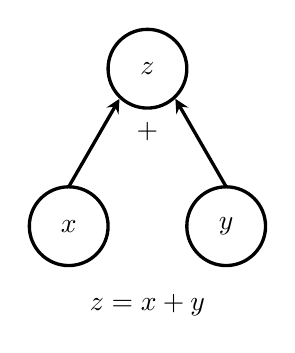
\begin{tikzpicture}
    % Result
    \draw [very thick] (1, 2) circle [radius=0.5cm] node {$z$};

    % Input Nodes
    \draw [very thick] (0, 0) circle [radius=0.5cm] node {$x$};
    \draw [very thick] (2, 0) circle [radius=0.5cm] node {$y$};

    % Edges
    \draw [very thick, -stealth] (0, 0.5) -- ++(60:1.29);
    \draw [very thick, -stealth] (2, 0.5) -- ++(120:1.29);

    % Operation Label
    \draw (1, 1.2) node {$+$};

    % Figure Label
    \draw (1, -1) node {$z = x + y$};
  \end{tikzpicture}
  %
  \hspace{0.2cm}
  %
  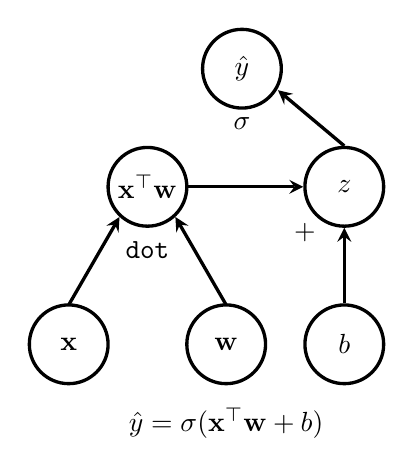
\begin{tikzpicture}
    % x^T w
    \draw [very thick] (1, 2) circle [radius=0.5cm] node {$\mathbf{x^\top w}$};

    % x and weights
    \draw [very thick] (0, 0) circle [radius=0.5cm] node {$\mathbf{x}$};
    \draw [very thick] (2, 0) circle [radius=0.5cm] node {$\mathbf{w}$};

    % Edges
    \draw [very thick, -stealth] (0, 0.5) -- ++(60:1.29);
    \draw [very thick, -stealth] (2, 0.5) -- ++(120:1.29);

    % Operation Label
    \draw (1, 1.2) node {\texttt{dot}};

    % Bias
    \draw [very thick] (3.5, 0) circle [radius=0.5cm] node {$b$};

    % z = (x^T w) + b
    \draw [very thick] (3.5, 2) circle [radius=0.5cm] node {$z$};

    % Operation label
    \draw (3, 1.42) node {$+$};

    % Edges
    \draw [very thick, -stealth] (3.5, 0.52) -- (3.5, 1.48);
    \draw [very thick, -stealth] (1.52, 2) -- (2.98, 2);

    % Sigmoid
    \draw [very thick] (2.2, 3.5) circle [radius=0.5] node {$\hat{y}$};

    % Operation label
    \draw (2.2, 2.8) node {$\sigma$};

    % Edge
    \draw [very thick, -stealth] (3.5, 2.52) -- ++(140:1.1cm);


    % Figure Label
    \draw (2, -1) node {$\hat{y} = \sigma(\mathbf{x}^\top \mathbf{w} + b)$};
  \end{tikzpicture}
  \label{fig:graphs}
  \caption{Examples of computational graphs. The left graph displays a very
    simple computation, consisting of just an addition of the two input
    variables $x$ and $y$. In this case, $z$ is the result of the operation $+$,
    as the annotation suggests. The right graph shows a more complex example of
    computing a logistic regression variable $\hat{y}$ in dependence of some
    example vector $\mathbf{x}$, weight vector $\mathbf{w}$ as well as a scalar
    bias $b$. As can be seen in the graph, $\hat{y}$ is the result of the
    \emph{sigmoid} function $\sigma$, also known as the \emph{logistic}
    function.}
\end{figure}

\subsubsection{Operations}\label{sec:model-graphs-ops}

The major benefit of representing an algorithm in form of a graph is not only
the intuitive (visual) expression of dependencies between units of a
computational model, but also the fact that the definition of a \emph{node}
within the graph can be kept very general. In TensorFlow, nodes represent
\emph{operations}, which in turn express the combination or transformation of
data flowing through the graph \cite{tensorflow}. An operation can have
\emph{zero or more} inputs and produce \emph{zero or more} outputs. As such, an
operation may represent a mathematical equation, a variable or constant, a
control-flow directive, a file I/O operation or even a network communication
port. It may seem unintuitive that an operation, which the reader may associate
with a \emph{function} in the mathematical sense, can represent a constant or
variable. However, a constant may be thought of as an operation that takes no
inputs and always produces the same output corresponding to the constant it
represents. Analogously, a variable is really just an operation taking no input
and producing the current state or value of that variable. Table \ref{tab:ops}
gives an overview of different kinds of operations that may be declared in a
TensorFlow graph.

\begin{table}
  \begin{tabular}{ll}
    \textbf{Category} & \textbf{Examples}
    \\ \toprule
    Elementwise operations & \texttt{Add}, \texttt{Mul}, \texttt{Exp}
    \\
    Matrix operations & \texttt{MatMul}, \texttt{MatrixInverse}
    \\
    Value-producing operations & \texttt{Constant}, \texttt{Variable}
    \\
    Neural-network units & \texttt{SoftMax}, \texttt{ReLU}, \texttt{Conv2D}
    \\
    Checkpoint operations & \texttt{Save}, \texttt{Restore}
    \end{tabular}
    \label{tab:ops}
    \caption{Examples for TensorFlow operations \cite{tensorflow}.}
\end{table}

Any operation must be backed by an associated implementation. In
\cite{tensorflow} such an implementation is referred to as the operation's
\emph{kernel}. A particular kernel is always specifically built for execution on
a certain kind of device, such as a CPU, GPU or other hardware unit.

\subsubsection{Tensors}\label{sec:model-graphs-tensors}

In Tensorflow, edges represent data flowing from one operation to another and
are referred to as \emph{tensors}. A tensor is a multi-dimensional collection of
homogenous values with a fixed, static type. The number of dimensions of a
tensor is termed its \emph{rank}. A tensor's \emph{shape} is the tuple
describing the size, i.e. the number of components, of the tensor in each
dimension. In the mathematical sense, a tensor is the generalization of
two-dimensional matrices, one-dimensional vectors and also scalars, which are
simply tensors of rank zero.

In terms of the computational graph, a tensor can be seen as a \emph{symbolic
  handle} to one of the outputs of an operation. A tensor itself does not hold
or store values in memory, but provides only an interface for retrieving the
value referenced by the tensor. When creating an operation in the TensorFlow
programming environment, such as for the expression $x + y$, a tensor object is
returned. This tensor may then be supplied as input to other computations,
thereby connecting the source and destination operations with an edge. By these
means, data flows through a TensorFlow graph.

Next to regular tensors, TensorFlow also provides a \texttt{SparseTensor}
data-structure, allowing for a more space-efficient dictionary-like
representation of \emph{sparse tensors} with only few non-zeros entries.

\subsubsection{Variables}\label{sec:model-graphs-vars}

In a typical situation, such as when performing stochastic gradient descent
(SGD), the graph of a machine-learning model is executed from start to end
multiple times for a single experiment. Between two such invocations, the
majority of tensors in the graph are destroyed and do not persist. However, it
is often necessary to maintain state across evaluations of the graph, such as
for the weights and parameters of a neural-network. Most often, one wishes to
update or \emph{train} this shared state either manually or as part of the
execution of the graph. For this purpose, there exist \emph{variables} in
TensorFlow, which are simply special operations that can be added to the
computational graph.

In detail, variables can be described as persistent, mutable handles to
in-memory buffers storing tensors. As such, variables are characterized by a
certain shape and a fixed type. To manipulate and update variables manually (as
opposed to implicitly by certain library routines), TensorFlow provides the
\texttt{assign} family of graph operations.

When creating a variable node for a TensorFlow graph, one must always supply a
tensor with which the variable is initialized upon graph execution. The shape
and data-type of the variable is then deduced from this
initializer. Interestingly, the variable iself does not store this initial
tensor. Rather, constructing a variable results in the addition of \emph{three}
distinct nodes to the graph:

\begin{enumerate}
  \item The actual variable node, holding the mutable state.
  \item An operation producing the initial value, often a constant.
  \item An \emph{initializer} operation, that \texttt{assign}s the initial value
    to the variable tensor upon evaluation of the graph.
\end{enumerate}

An example for this is given in Figure \ref{fig:variable}.

\begin{figure}
  \centering
    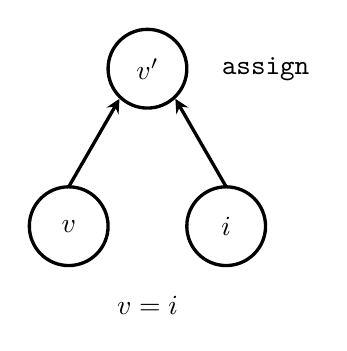
\begin{tikzpicture}
    % Result
    \draw [very thick] (1, 2) circle [radius=0.5cm] node {$v'$};

    % Input Nodes
    \draw [very thick] (0, 0) circle [radius=0.5cm] node {$v$};
    \draw [very thick] (2, 0) circle [radius=0.5cm] node {$i$};

    % Edges
    \draw [very thick, -stealth] (0, 0.5) -- ++(60:1.29);
    \draw [very thick, -stealth] (2, 0.5) -- ++(120:1.29);

    % Operation Label
    \draw (2.5, 2) node {\texttt{assign}};

    % Figure Label
    \draw (1, -1) node {$v = i$};
  \end{tikzpicture}
  \label{fig:variable}
  \caption{The three nodes that are added to the computational graph for every
    variable definition. The first, $v$, is the variable operation that holds a
    mutable in-memory buffer containing the value-tensor of the variable. The
    second, $i$, is the node producing the initial value for the variable, which
    can be any tensor (that is, the result of any operation). Lastly, the
    \texttt{assign} node will set the variable to the initializer's value when
    executed. The \texttt{assign} node also produces a tensor referencing the
    initialized value $v'$ of the variable, such that it may be connected to
    other nodes as necessary (e.g. when using a variable as the initializer for
    another variable). }
\end{figure}

\subsubsection{Sessions}\label{sec:model-graphs-sessions}

In TensorFlow, the execution of operations and the evalution of tensors may only
be performed in a special environment referred to as \emph{session}. One of the
responsibilities of a session is to encapsulate the allocation and management of
resources such as variable buffers. Moreover, the \texttt{Session} interface of
the TensorFlow library provides a \texttt{run} routine, which is the primary
entry-point for executing parts or the entirety of a computational graph. This
method takes as input the nodes in the graph whose tensors should be computed
and returned. Moreover, an optional mapping from arbitrary nodes in the graph to
respective replacement values --- referred to as \emph{feed nodes} --- may be
supplied to \texttt{run} as well \cite{tensorflow}.

Upon invocation of \texttt{run}, TensorFlow will start at the requested output
nodes and work backwards, examining the graph dependencies and computing the
full transitive closure of all nodes that must be executed. These nodes may then
be assigned to one or many physical execution units (CPUs, GPUs etc.) on one or
many machines. The rules by which this assignment takes place are determined by
TensorFlow's \emph{placement algorithm}, discussed in detail in Subsection
\ref{subsec:execmodel}, Moreover, as there exists the possibility to specify
explicit orderings of node evaluations, called \emph{control dependencies}, the
execution algorithm will ensure that these dependencies are maintained.

\subsection{Execution Model}\label{sec:model-exec}

To execute computational graphs composed of the various elements just discussed,
TensorFlow divides the tasks of its implementation among four distinct groups:
the \emph{client}, the \emph{master}, a set of \emph{workers} and lastly a
number of \emph{devices}. When the client requests evaluation of a TensorFlow
graph via a \texttt{Session}'s \texttt{run} routine, this query is sent to the
master process, which in turn delegates the task to one or more worker processes
and coordinates their execution. Each worker is subsequently responsible for
overseeing one or more devices, which are the physical processing units for
which the kernels of an operation are implemented.

Within this model, there are two degrees of scalability. The first degree
pertains to scaling the number of machines on which a graph is executed. The
second degree refers to the fact that on each machine, there may then be more
than one device, such as, for example, five independent GPUs and/or three
CPUs. For this reason, there exist two ``versions'' of TensorFlow, one for local
execution on a single machine (but possibly many devices), and one supporting a
\emph{distributed} implementation across many machines and many devices in a
cluster. Figure \ref{fig:exec} visualizes a possible distributed setup. Since 13
April 2016, the distributed version of TensorFlow is also part of its
open-source distribution \cite{tensorflowdist}.

\begin{figure}
  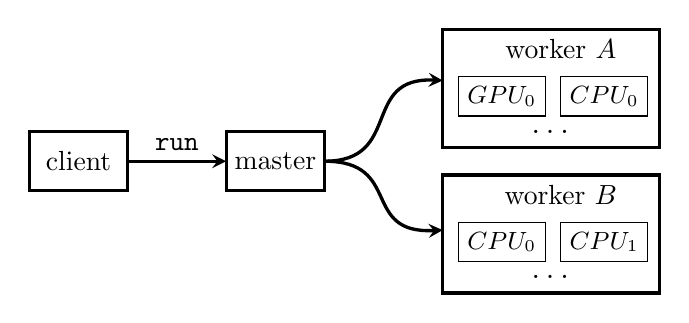
\begin{tikzpicture}
    % Client
    \draw [very thick] (0, 0) rectangle ++(1.25, 0.75) node [midway] {client};

    % Master
    \draw [very thick] (2.5, 0) rectangle ++(1.25, 0.75) node [midway] {master};
    \draw [very thick, -stealth] (1.25, 0.375) -- (2.5, 0.375) node [midway,
    above] {\texttt{run}};

    % Worker 1
    \draw [very thick] (5.25, 0.55) rectangle ++(2.75, 1.5);
    \draw (6.75, 1.8) node {worker $A$};
    \draw (5.45, 0.95) rectangle ++(1.1, 0.5) node [midway] {\small$GPU_0$};
    \draw (6.75, 0.95) rectangle ++(1.1, 0.5) node [midway] {\small$CPU_0$};
    \draw (6.65, 0.75) node {\large\dots};


    % Worker 2
    \draw [very thick] (5.25, -1.3) rectangle ++(2.75, 1.5);
    \draw (6.75, -0.05) node {worker $B$};
    \draw (5.45, -0.9) rectangle ++(1.1, 0.5) node [midway] {\small$CPU_0$};
    \draw (6.75, -0.9) rectangle ++(1.1, 0.5) node [midway] {\small$CPU_1$};
    \draw (6.65, -1.1) node {\large\dots};

    % Edges
    \draw [very thick, -stealth]
          (3.75, 0.375) .. controls +(1, 0) and (4.2, 1.45) .. (5.25, 1.4);
    \draw [very thick, -stealth]
          (3.75, 0.375) .. controls +(1, 0) and (4.2, -0.55) .. (5.25, -0.5);

  \end{tikzpicture}
  \label{fig:exec}
  \caption{A visualization of the different execution agents in a multi-machine,
    multi-device hardware configuration.}
\end{figure}

\subsubsection{Devices}\label{sec:model-exec-devices}

Devices are the smallest, most basic entities in the TensorFlow execution
model. All nodes in the graph, that is, the kernel of each operation, must
eventually be mapped to an available device to be executed. In practice, a
device will most often be either a CPU or a GPU. However, TensorFlow supports
registration of additional types of \emph{physical execution units} by the
user. For example, in May 2016, Google announced its \emph{Tensor Processing
  Unit} (TPU), which is a custom-built ASIC
(application-specific-integrated-circuit) optimized specifically for fast
tensor-computations \cite{tpu}. It is thus understandibly easy to integrate new
device classes as novel hardware emerges.

To oversee the evaluation of nodes on a device, a worker process is spawned by
the master. As a worker process may manage one or many devices on a single
machine, a device is identified not only by a name, but also an index for its
worker group. For example, the first CPU in a particular group may be identified
by the string ``/cpu:0''.

\subsubsection{Placement Algorithm}\label{sec:model-exec-placement}

To determine which nodes to assign to which device, TensorFlow makes use of a
\emph{placement algorithm}. The placement algorithm simulates the execution of
the computational graph and traverses its nodes from input tensors to output
tensors. To decide on which of the available devices
$\mathbb{D} = \{d_1, \dots, d_n\}$ to place a given node $\nu$ encountered
during this traversal, the algorithm consults a \emph{cost model}
$C_\nu(d)$. This cost model takes into account four pieces of information to
determine the optimal device $\hat{d} = \argmin_{d \in \mathbb{D}} C_\nu(d)$ on
which to place the node during execution:

\begin{enumerate}
  \item Whether or not there exists an implementation (kernel) for a node on the
    given device at all. For example, if there is no GPU kernel for a particular
    operation, any GPU device would automatically incur an infinite cost.
  \item Estimates of the size (in bytes) of the input and output tensors of the
    node.
  \item The expected execution time for the kernel on the device.
  \item A heuristic for the cost of cross-device (and possibly cross-machine)
    transmission of the input tensors to the operation, in the case that the
    input tensors have been placed on nodes different from the one currently
    under consideration.
\end{enumerate}

\subsubsection{Cross-Device Execution}\label{sec:model-exec-single}

If the hardware configuration of the user's system provided more than one
device, the placement algorithm will often have distributed the graph nodes
among these devices. This can be seen as partitioning the set of nodes into
classes, one per device. As a consequence, there may be cross-device
dependencies between nodes that must be handled via a number of additional
steps. Let us consider for this two devices $A$ and $B$ with particular focus on
a node $\nu$ on device $A$. If $\nu$'s output tensor forms the input to some
other operations $\alpha, \beta$ on device $B$, there initially exists
cross-device edges $\nu \rightarrow \alpha$ and $\nu \rightarrow \beta$ from
device $A$ to device $B$. This is visualized in Figure \ref{fig:cross-a}.

In practice, there must be some means of transmitting $\nu$'s output tensor from
$A$, say a GPU device, to $B$, maybe a CPU device. For this reason, TensorFlow
initially replaces the two edges by three new nodes and an additional edge. On
device $A$, a \texttt{send}-node is placed and connected to $\nu$. In tandem, on
device $B$, two \texttt{recv}-node are instantiated and connected to $\alpha$
and $\beta$, respectively. The \texttt{send} and \texttt{recv} nodes are then
connected by new edges. This step is shown in Figure \ref{fig:cross-b}. During
execution of the graph, cross-device communication of data occurrs exclusively
via these special nodes. If the devices are on the same machine, the
transmission will most likely occur over a PCI Express bus. When the devices are
located on separate machines, the transmission between the worker processes on
these machines may involve remote communication protocols such as TCP or RDMA.

Finally, an important optimization made by TensorFlow at this step is
``canonicalization'' of $(\mathtt{send}, \mathtt{receive})$ pairs. In the setup
displayed in Figure \ref{fig:cross-b}, the existence of each \texttt{recv} node
on device $B$ would imply allocation and management of a separate buffer to
store $\nu$'s output tensor, so that it may then be fed to nodes $\alpha$ and
$\beta$, respectively. However, an equivalent and much more efficient
transformation places only one \texttt{recv} node on device $B$ and streams all
output from $\nu$ to this single node, and then to the two dependent nodes
$\alpha$ and $\beta$. This last and final evolution is given in Figure
\ref{fig:cross-c}.

\begin{figure}
  \centering
  %
  \begin{subfigure}[b]{0.30\textwidth}
    \centering
    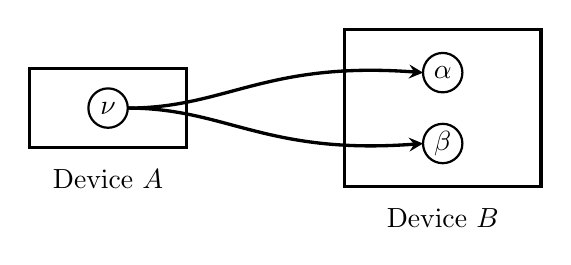
\begin{tikzpicture}
      % Device A
      \draw [very thick] (0, 0) rectangle (2, 1);
      \draw (1, -0.4) node {Device $A$};
      \draw [thick] (1, 0.5) circle [radius=0.25] node {$\nu$};

      % Device B
      \draw [very thick] (4, -0.5) rectangle (6.5, 1.5);
      \draw (5.25, -0.9) node {Device $B$};
      \draw [thick] (5.25, 0.05) circle [radius=0.25] node {$\beta$};
      \draw [thick] (5.25, 0.95) circle [radius=0.25] node {$\alpha$};

      % Edges
      % nu -> beta
      \draw [very thick, -stealth] (1.25, 0.5)
            .. controls (2.5, 0.5) and (3, 1.1)
            ..         (5, 0.95);
      % nu -> alpha
      \draw [very thick, -stealth] (1.25, 0.5)
            .. controls (2.5, 0.5) and (3, -0.1)
            ..          (5, 0.05);
    \end{tikzpicture}
    \label{fig:cross-a}
    \caption{}
  \end{subfigure}
  %
  \begin{subfigure}[b]{0.30\textwidth}
    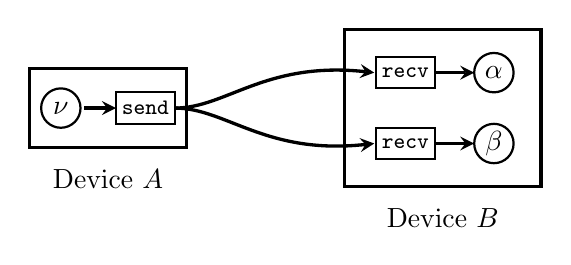
\begin{tikzpicture}
      % Device A
      \draw [very thick] (0, 0) rectangle (2, 1);
      \draw (1, -0.4) node {Device $A$};
      \draw [thick] (0.4, 0.5) circle [radius=0.25] node {$\nu$};

      % Device B
      \draw [very thick] (4, -0.5) rectangle (6.5, 1.5);
      \draw (5.25, -0.9) node {Device $B$};
      \draw [thick] (5.9, 0.05) circle [radius=0.25] node {$\beta$};
      \draw [thick] (5.9, 0.95) circle [radius=0.25] node {$\alpha$};

      % Send Nodes
      \draw [thick] (1.1, 0.3) rectangle ++(0.75, 0.4) node [midway]
      {\footnotesize\texttt{send}};
      \draw [very thick, -stealth] (0.7, 0.5) -- (1.1, 0.5);

      % Receive Nodes
      \draw [thick] (4.4, 0.75) rectangle ++(0.75, 0.4) node [midway]
      {\footnotesize\texttt{recv}};
      \draw [very thick, -stealth] (5.15, 0.95) -- ++(0.5, 0);
      \draw [thick] (4.4, -0.15) rectangle ++(0.75, 0.4) node [midway]
      {\footnotesize\texttt{recv}};
      \draw [very thick, -stealth] (5.15, 0.05) -- ++(0.5, 0);

      % Edges
      % nu -> beta
      \draw [very thick, -stealth] (1.85, 0.5)
            .. controls (2.5, 0.5) and (3, 1.1)
            ..         (4.38, 0.95);
      % nu -> alpha
      \draw [very thick, -stealth] (1.85, 0.5)
            .. controls (2.5, 0.5) and (3, -0.1)
            ..          (4.38, 0.05);
    \end{tikzpicture}
    \label{fig:cross-b}
    \caption{}
  \end{subfigure}
  %
  \begin{subfigure}[h]{0.30\textwidth}
    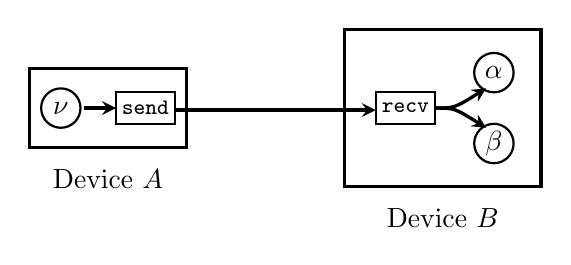
\begin{tikzpicture}
            % Device A
      \draw [very thick] (0, 0) rectangle (2, 1);
      \draw (1, -0.4) node {Device $A$};
      \draw [thick] (0.4, 0.5) circle [radius=0.25] node {$\nu$};

      % Device B
      \draw [very thick] (4, -0.5) rectangle (6.5, 1.5);
      \draw (5.25, -0.9) node {Device $B$};
      \draw [thick] (5.9, 0.05) circle [radius=0.25] node {$\beta$};
      \draw [thick] (5.9, 0.95) circle [radius=0.25] node {$\alpha$};

      % Send Nodes
      \draw [thick] (1.1, 0.3) rectangle ++(0.75, 0.4) node [midway]
      {\footnotesize\texttt{send}};
      \draw [very thick, -stealth] (0.7, 0.5) -- (1.1, 0.5);

      % Receive Nodes
      \draw [thick] (4.4, 0.3) rectangle ++(0.75, 0.4) node [midway]
      {\footnotesize\texttt{recv}};
      \draw [very thick, -stealth] (5.15, 0.5)
                      .. controls +(0.25, 0)
                               .. +(0.65, 0.25);
      \draw [very thick, -stealth] (5.15, 0.5)
                      .. controls +(0.25, 0)
                               .. +(0.65, -0.25);

      % Edges
      \draw [very thick, -stealth] (1.85, 0.475) -- (4.4, 0.475);
    \end{tikzpicture}
    \label{fig:cross-c}
    \caption{}
  \end{subfigure}
  \label{fig:cross}
  \caption{The three stages of cross-device communication between graph nodes in
    TensorFlow. Figure \ref{fig:cross-a} shows the initial, conceptual
    connections between nodes on different devices. Figure \ref{fig:cross-b}
    gives a more practical overview of how data is actually transmitted across
    devices using \texttt{send} and \texttt{recv} nodes. Lastly, Figure
    \ref{fig:cross-c} shows the final, canonicalized setup, where there is at
    most one \texttt{recv} node per destination device.}
\end{figure}

\subsection{Optimizations}\label{sec:model-optim}

To ensure a maximum of efficiency and performance of the TensorFlow execution
model, a number of optimizations are built into the library. In this subsection,
we examine three such improvements: common subgraph elimination, execution
scheduling and finally lossy compression.

\subsubsection{Common-Subgraph Elimination}\label{sec:model-optim-common}

An optimzation performed by many modern compilers is \emph{common subexpression
  elimination}, whereby a compiler may possibly replace the computation of an
identical value two or more times by a single instance of that computation. The
result is then stored in a temporary variable and reused where it was previously
re-calculated. Similarly, in a TensorFlow graph, it may occur that the same
operation is performed on identical inputs more than once. This can be
inefficient if the computation happens to be an expensive one. Moreover, it may
incur a large memory overhead given that the result of that operation must be
held in memory multiple times. Therefore, TensorFlow also employs a
common-subexpression, or, more aptly put, common \emph{subgraph} elimination
pass prior to execution. For this, the computational graph is traversed and
every time two or more operations of the same type (e.g. \texttt{MatMul})
receiving the same input tensors are encountered, they are canoncalized to only
one such subgraph. The output tensor of that single operation is then redirected
to all dependent nodes. Figure \ref{fig:subgraph-elim} gives an example of
common subgraph elimination.

\begin{figure}
  \centering
  \begin{subfigure}[h]{0.5\textwidth}
    \centering
    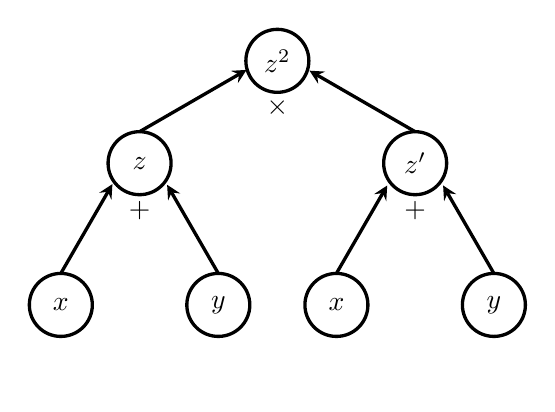
\begin{tikzpicture}
      % First operation
      \draw [very thick] (1, 1.8) circle [radius=0.4cm] node {$z$};

      % Input Nodes
      \draw [very thick] (0, 0) circle [radius=0.4cm] node {$x$};
      \draw [very thick] (2, 0) circle [radius=0.4cm] node {$y$};

      % Edges
      \draw [very thick, -stealth] (0, 0.4) -- ++(60:1.31);
      \draw [very thick, -stealth] (2, 0.4) -- ++(120:1.3);

      % Operation Label
      \draw (1, 1.2) node {$+$};

      % Second operation
      \draw [very thick] (4.5, 1.8) circle [radius=0.4cm] node {$z'$};

      % Input Nodes
      \draw [very thick] (3.5, 0) circle [radius=0.4cm] node {$x$};
      \draw [very thick] (5.5, 0) circle [radius=0.4cm] node {$y$};

      % Edges
      \draw [very thick, -stealth] (3.5, 0.4) -- ++(60:1.29);
      \draw [very thick, -stealth] (5.5, 0.4) -- ++(120:1.29);

      % Operation Label
      \draw (4.5, 1.2) node {$+$};

      % Square
      \draw [very thick] (2.75, 3.1) circle [radius=0.4cm] node {$z^2$};

      % Edges
      \draw [very thick, -stealth] (1, 2.2) -- ++(30:1.57);
      \draw [very thick, -stealth] (4.5, 2.2) -- ++(150:1.55);

      % Operation Label
      \draw (2.75, 2.5) node {$\times$};

      % Spacing fuck you
      \draw (0, -1);
    \end{tikzpicture}
  \end{subfigure}
  %
  \begin{subfigure}[h]{0.5\textwidth}
    \centering
    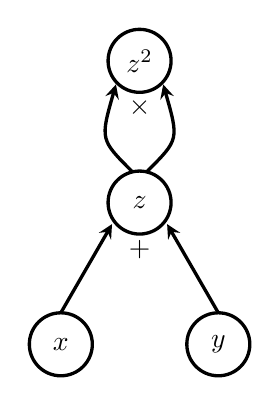
\begin{tikzpicture}
      % First operation
      \draw [very thick] (1, 1.8) circle [radius=0.4cm] node {$z$};

      % Input Nodes
      \draw [very thick] (0, 0) circle [radius=0.4cm] node {$x$};
      \draw [very thick] (2, 0) circle [radius=0.4cm] node {$y$};

      % Edges
      \draw [very thick, -stealth] (0, 0.4) -- ++(60:1.3);
      \draw [very thick, -stealth] (2, 0.4) -- ++(120:1.3);

      % Operation Label
      \draw (1, 1.2) node {$+$};

      % Square
      \draw [very thick] (1, 3.6) circle [radius=0.4cm] node {$z^2$};

      % Operation Label
      \draw (1, 3) node {$\times$};

      % Edges
      \draw [very thick, -stealth] (0.9, 2.2) .. controls +(-0.4, 0.4) .. +(-0.2, 1.1);
      \draw [very thick, -stealth] (1.1, 2.2) .. controls +(+0.4, 0.4) .. +(+0.2, 1.1);
    \end{tikzpicture}
  \end{subfigure}
  %
  \label{fig:subgraph-elim}
  \caption{An example of how common-subgraph elimination is used to transorm the
    equations $z = x + y$, $z' = x + y$, $z^2 = z \cdot z'$ to just two
    equations $z = x + y$ and $z^2 = z \cdot z$. This computation could
    theoretically be optimized further to a \texttt{square} operation requiring
    only one input (thus reducing the cost of data movement), though it is not
    known if TensorFlow employs such secondary canonicalization.}
\end{figure}

\subsubsection{Scheduling}\label{sec:model-optim-schedule}

A simple yet powerful optimization is to schedule node execution as late as
possible. Ensuring that the results of operations remain in memory only for the
minimum required amount of time reduces peak memory consumption and can thus
greatly improve the overall performance of the system. The authors of
\cite{tensorflow} note that this is especially vital on devices such as GPUs,
where memory resources are scarce. Furthermore, careful scheduling also pertains
to the activation of \texttt{send} and \texttt{recv} nodes, where not only
memory but also network resources are contested.

\subsubsection{Lossy Compression}\label{sec:model-optim-lossy}

One of the primary goals of many machine-learning algorithms used for
classification, recognition or other tasks is to build robust models. With
\emph{robust} we mean that an optimally trained model should ideally not change
its response if it is first fed a signal and then a noisy variaton of that
signal. As such, these machine-learning algorithms typically do not require high
precision arithmetic as provided by standard IEEE 754 32-bit floating point
values. Rather, 16 bits of precision in the mantissa would do just as well. For
this reason, another optimization performed by TensorFlow is the internal
addition of conversion nodes to the computational graph, which convert such
high-precision 32-bit floating-point values to truncated 16-bit representations
when communicating across devices and across machines. On the receiving end, the
truncated representation is converted back to 32 bits simply by filling in
zeros, rather than rounding \cite{tensorflow}.

\subsection{Additions to the Basic Programming Model}\label{sec:model-ext}

Having discussed the basic computation and execution model of TensorFlow, we
will now review three more advanced topics that we deem highly relevant for
anyone wishing to use TensorFlow to create machine-learning algorithms. First,
we will discuss how TensorFlow handles \emph{gradient backpropagation}, an
essential concept for many deep-learning applications. Then, we will discuss in
what way TensorFlow graphs support \emph{control-flow}. Lastly, we briefly touch
upon the topic of \emph{checkpoints}, as they are very useful for maintenance of
large models.

\subsubsection{Back-Propagation Nodes}\label{sec:model-ext-backprop}

In a large number of deep-learning and other machine-learning algorithms, it is
necessary to compute the gradients of particular nodes of the computational
graph with respect to one or many other nodes. For example, in a neural network,
we may compute the cost $c$ of the model for a given example $x$ by passing that
example through a series of non-linear transformations. If the neural network
consists of two hidden layers, represented by functions $f$ and $g$, we can
express the cost for that example as $c = (f \circ g)(x) = f(g(x))$. We would
then typically wish to calculate the gradient $dc/dx$ of that cost with respect
to the input value $x$ and use it to update certain internal
parameters. Usually, we would do this by means of the \emph{back-propagation}
algorithm, which traverses the graph in reverse to compute the chain rule
$[f(g(x))]' = f'(g(x)) \cdot g'(x)$.

In \cite{goodfellow2016}, two approaches for back-propagating gradients through
a computational graph are described. The first, which the authors refer to as
\emph{symbol-to-number differentiation}, receives a set of input values and then
computes the \emph{numerical values} of the gradients at those input values. It
does so by explicitly traversing the graph first in the forward order
(forward-propagation) to compute the cost, then in reverse order
(back-propagation) to compute the gradients via the chain rule. Another
approach, more relevant to TensorFlow, is what \cite{goodfellow2016} calls
\emph{symbol-to-symbol derivatives} and \cite{tensorflow} terms \emph{automatic
  gradient computation}. In this case, gradients are not computed by an explicit
implementation of the backpropagation algorithm. Rather, special nodes are added
to the computational graph that calculate the gradient of each operation and
thus ultimately the chain rule. To perform back-propagation, these nodes must
then simply be executed like any other nodes by the graph evaluation engine. As
such, this approach does not produce the desired derivatives as a numeric value,
but only as a \emph{symbolic handle} to compute those values.

When TensorFlow needs to compute the gradient of a particular node $\nu$ (that
is, the tensor produced by that operation) with respect to some other tensor
$\alpha$, it traverses the graph in reverse order from $\nu$ to $\alpha$. Each
operation $o$ encountered during this traversal represents a function depending
on $\alpha$ and is one of the ``links'' in the chain
$(\nu \,\circ\, \dots\, o \,\circ\, \dots)(\alpha)$ producing the output tensor
of the graph. Therefore, TensorFlow adds a \emph{gradient node} for each such
operation $o$ that takes the gradient of the previous link (the outer function)
and multiplies it with its gradient $\frac{do}{d\alpha}$. At the end of the
traversal, there will be a node providing a symbolic handle to the overall
target derivative $\frac{d\nu}{d\alpha}$. It should now be clear that
back-propagation in this symbol-to-symbol approach is implemented just like
\emph{any other computation} and requires no exceptional handling. Figure
\ref{fig:gradients} shows how a computational graph may look before and after
gradient nodes are added.

\begin{figure}
  \centering
  \begin{subfigure}[b]{0.2\textwidth}
    \centering
    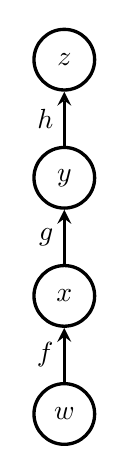
\begin{tikzpicture}
      % Nodes
      \path [very thick] (0, 0)
            coordinate [draw, circle, text width=0.5cm] (w) node {$w$};
      \path [very thick] (0, 1.5)
             coordinate [draw, circle, text width=0.5cm] (x) node {$x$};
      \path [very thick] (0, 3)
            coordinate [draw, circle, text width=0.5cm] (y) node {$y$};
      \path [very thick] (0, 4.5)
            coordinate [draw, circle, text width=0.5cm] (z) node {$z$};

      % Edges
      \draw [very thick, -stealth] (w) -- (x) node [midway, left] {$f$};
      \draw [very thick, -stealth] (x) -- (y) node [midway, left] {$g$};
      \draw [very thick, -stealth] (y) -- (z) node [midway, left] {$h$};
    \end{tikzpicture}
    \caption{}
    \label{fig:gradients-a}
  \end{subfigure}
  \begin{subfigure}[b]{0.2\textwidth}
    \centering
    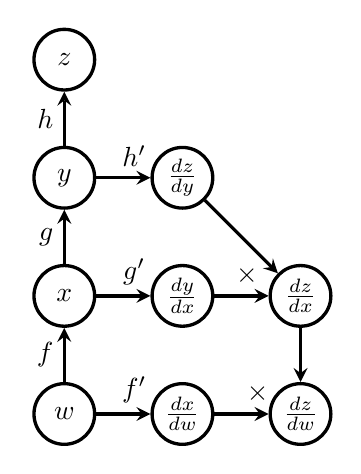
\begin{tikzpicture}
      % Nodes
      \path [very thick] (0, 0)
            coordinate [draw, circle, text width=0.5cm] (w) node {$w$};
      \path [very thick] (0, 1.5)
             coordinate [draw, circle, text width=0.5cm] (x) node {$x$};
      \path [very thick] (0, 3)
            coordinate [draw, circle, text width=0.5cm] (y) node {$y$};
      \path [very thick] (0, 4.5)
            coordinate [draw, circle, text width=0.5cm] (z) node {$z$};

      % Edges
      \draw [very thick, -stealth] (w) -- (x) node [midway, left] {$f$};
      \draw [very thick, -stealth] (x) -- (y) node [midway, left] {$g$};
      \draw [very thick, -stealth] (y) -- (z) node [midway, left] {$h$};

      % Derivatives
      \path [very thick] (1.5, 0)
            coordinate [draw, circle, text width=0.5cm] (wp) node {$\frac{dx}{dw}$};
      \path [very thick] (1.5, 1.5)
             coordinate [draw, circle, text width=0.5cm] (xp) node {$\frac{dy}{dx}$};
      \path [very thick] (1.5, 3)
            coordinate [draw, circle, text width=0.5cm] (yp) node {$\frac{dz}{dy}$};

      % Edges
      \draw [very thick, -stealth] (w) -- (wp) node [pos=0.7, above] {$f'$};
      \draw [very thick, -stealth] (x) -- (xp) node [pos=0.7, above] {$g'$};
      \draw [very thick, -stealth] (y) -- (yp) node [pos=0.7, above] {$h'$};

     % Chain Rule
      \path [very thick] (3, 0)
            coordinate [draw, circle, text width=0.5cm]
            (dzdw) node {$\frac{dz}{dw}$};
      \path [very thick] (3, 1.5)
             coordinate [draw, circle, text width=0.5cm]
             (dzdx) node {$\frac{dz}{dx}$};

      % Edges
      \draw [very thick, -stealth] (wp) -- (dzdw)
            node [pos=0.8, above] {$\times$};
      \draw [very thick, -stealth] (xp) -- (dzdx)
            node [pos=0.6, above] {$\times$};
      \draw [very thick, -stealth] (yp) -- (dzdx);
      \draw [very thick, -stealth] (dzdx) -- (dzdw);
    \end{tikzpicture}
    \caption{}
    \label{fig:gradients-b}
  \end{subfigure}
  \caption{A computational graph before (\ref{fig:gradients-a}) and after
    (\ref{fig:gradients-b}) gradient nodes are added. In this
    \emph{symbol-to-symbol} approach, the gradient $\frac{dz}{dw}$ is just
    simply an operation like any other and therefore requires no special
    handling by the graph evaluation engine.}
  \label{fig:gradients}
\end{figure}

In \cite{tensorflow} it is noted that symbol-to-symbol derivatives may incur a
considerable performance cost and especially result in increased memory
overhead. To see why, it is important to understand that there exist two
equivalent formulations of the chain rule. The first reuses previous
computations and is given in Equation \ref{eq:chain-reuse} for example functions
$f$, $g$ and $h$. The second was already shown, where each function recomputes
all of its arguments and invokes every function it depends on. It is given in
Equation \ref{eq:chain-recomp} for reference.

\begin{equation}\label{eq:chain-reuse}
  \frac{d f}{d w} = f'(y) \cdot g'(x) \cdot h'(w) \text{ with } y = g(x), x =
  h(w)
\end{equation}

\begin{equation}\label{eq:chain-recomp}
  \frac{d f}{d w} = f'(g(h(w))) \cdot g'(h(w)) \cdot h'(w)
\end{equation}

According to \cite{tensorflow}, TensorFlow currently employs the first
approach. Given that the inner-most functions must be recomputed for every link
of the chain if this approach is not employed, and taking into consideration
that this chain may consist of many hundreds or thousands of operations, this
choice seems sensible. However, on the flip side, keeping tensors in memory for
long periods of time is also not optimal, especially on devices like GPUs where
memory resources are scarce. For Equation \ref{eq:chain-recomp}, memory held by
tensors could in theory be freed as soon as it has been processed by its graph
dependencies. For this reason, in \cite{tensorflow} the development team of
TensorFlow states that recomputing certain tensors rather than keeping them in
memory may be a possible performance improvement for the future.

\subsubsection{Control-Flow}\label{sec:model-ext-flow}

Some machine-learning algorithms may benefit from being able to control the flow
of their execution, performing certain steps only under a particular condition
or repeating some computation a fixed or variable number of times. For this,
TensorFlow provides a set of control-flow primitives including
\texttt{if}-conditionals and \texttt{while}-loops. The possibility of loops is
the reason why a TensorFlow computational graph is not necessarily
\emph{acyclic}. If the number of iterations for of a loop would be fixed and
known at graph compile-time, its body could be \emph{unrolled} into an acyclic
sequence of computations, one per loop iteration \cite{theano}. However, to
support a variable amount of iterations, TensorFlow is forced to jump through an
additional set of hoops, as described in \cite{tensorflow}.

One aspect that must be especially cared for when introducing control-flow is
back-propagation. In the case of a conditional, where an \texttt{if}-operation
returns either one or the other tensor, its gradient node must be aware of which
branch the node took during forward-propagation. Moreover, when a loop body
(which may be a small graph) was executed a certain number of times, the
gradient computation does not only need to know the number of iterations
performed, but also requires access to each intermediary value produced. This
technique of stepping through a loop in reverse to compute the gradients is
referred to as \emph{back-propagation through time} in \cite{theano}.

\subsubsection{Checkpoints}\label{sec:model-ext-check}

A small additional extension to TensorFlow's basic programming model is the
notion of \emph{checkpoints}, which allow for serialization of variables and
storage on disk. It is possible to add \texttt{Store} nodes to the computational
graph and connect them to variables whose tensors you wish to save. Furthermore,
a variable may be connected to a \texttt{Restore} operation, which deserializes
a stored tensor at a later point. This is especially useful when training a
model over a long period of time to keep track of the model's performance as
time progresses while reducing the risk of losing any progress made. Also,
checkpoints are a vital element to ensuring fault-tolerance in a distributed
environment \cite{tensorflow}.

%%% Local Variables:
%%% mode: latex
%%% TeX-master: "../paper"
%%% End:
\section{The TensorFlow Programming Interface}\label{sec:code}

\subsection{Interfaces}\label{sec:code-interfaces}

\subsection{Walkthrough}\label{sec:code-walk}

\subsection{Abstractions}\label{sec:code-abstract}

%%% Local Variables:
%%% mode: latex
%%% TeX-master: "../paper"
%%% End:
\section{Comparison With Other Deep-Learning Frameworks}\label{sec:comp}
\section{Comparison With Other Deep Learning Frameworks}\label{sec:comp}

Next to TensorFlow, there exist a number of other open source deep learning
software libraries, the most popular being Theano, Torch and Caffe. In this
section, we review two sources of quantitative comparisons between TensorFlow
and these alternatives, providing a summary of the most important results of
each work.

The first source in our collection is the \emph{convnet-benchmarks} repository
on GitHub by Soumith Chintala \cite{convnet-bench}, a research engineer at
Facebook. The commit we reference\footnote{Commit hash:
  84b5bb1785106e89691bc0625674b566a6c02147} is dated April 25, 2016. Chintala
provides an extensive set of benchmarks for a variety of convolutional network
models and many libraries. Inter alia, Chintala gives the forward and
backward-propagation time of TensorFlow, Torch and Caffe for the AlexNet CNN
model \cite{alexnet}. Theano is not included in these benchmarks. The outcomes
show that TensorFlow performs second-best in both measures behind Torch, with
Caffe lagging relatively far behind. We reproduce the relevant results in Table
\ref{tab:convnet}.

\begin{table}
  \centering
  \begin{tabular}{ccc}
    \textbf{Library} & \textbf{Forward (ms)} & \textbf{Backward (ms)}
    \\ \toprule
    TensorFlow & 26  & 55
    \\
    Torch & \textbf{25} & \textbf{46}
    \\
    Caffe & 121 & 203
    \\ \bottomrule
  \end{tabular}
  \caption{The result of Soumith Chintala's benchmarks for TensorFlow, Torch and
    Caffe (not Theano) on an AlexNet ConvNet model \cite{alexnet,
      convnet-bench}.}
  \label{tab:convnet}
\end{table}

Further benchmarks were published by the Theano development team in
\cite{theano} on May 9, 2016. We focus on their results for an LSTM network
operating on the Penn Treebank dataset \cite{penntreebank}. Their comparisons
measure words processed per second for a small model consisting of a single
200-unit hidden layer and a large model with two 650-unit hidden layers. Tested
libraries include Theano, Torch and TensorFlow, but not Caffe. In their
benchmarks, TensorFlow performs best among all three for the small model,
followed by Theano and then Torch. For the large model, TensorFlow is placed
second behind Theano, while Torch remains in last place. Table
\ref{fig:theano-results} shows these outcomes.

\begin{figure}
  \centering
  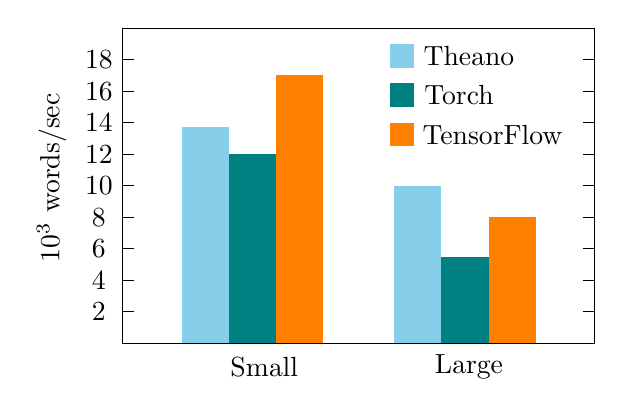
\begin{tikzpicture}
    % Frame
    \draw (0, 0) rectangle (6, 4);

    % Ticks + Scale
    \foreach \i in {2, 4, ..., 18} {
      % Left
      \draw (0, {\i / 5}) -- ++(+0.15, 0);
      % Right
      \draw (5.85, {\i / 5}) -- ++(+0.15, 0);
      % Labels
      \draw (-0.3, {\i / 5}) node {\i};
    }

    % Legend
    \draw (-0.9, 2.1) node [rotate=90] {$10^3$ words/sec};

    \fill [SkyBlue] (3.4, 3.5) rectangle ++(0.3, 0.3);
    \draw (4.4, 3.65) node {Theano};

    \fill [teal] (3.4, 3) rectangle ++(0.3, 0.3);
    \draw (4.275, 3.15) node {Torch};

    \fill [orange] (3.4, 2.5) rectangle ++(0.3, 0.3);
    \draw (4.7, 2.65) node {TensorFlow};


    %%% Small Model %%%

    % Theano
    \fill [SkyBlue] (0.75, 0) rectangle ++(0.6, 2.75);
    % Torch
    \fill [teal] (1.35, 0) rectangle ++(0.6, 2.4);
    % TensorFlow
    \fill [orange] (1.95, 0) rectangle ++(0.6, 3.4);

    % Label
    \draw (1.8, -0.3) node {Small};

    %%% Large Model %%%

    % Theano
    \fill [SkyBlue] (3.45, 0) rectangle ++(0.6, 2);
    % Torch
    \fill [teal] (4.05, 0) rectangle ++(0.6, 1.1);
    % TensorFlow
    \fill [orange] (4.65, 0) rectangle ++(0.6, 1.6);

    % Label
    \draw (4.4, -0.3) node {Large};

  \end{tikzpicture}
  \caption{The results of \cite{theano}, comparing TensorFlow, Theano and Torch
    on an LSTM model for the Penn Treebank dataset \cite{penntreebank}. On the
    left the authors tested a small model with a single hidden layer and 200
    units; on the right they use two layers with 650 units each. }
  \label{fig:theano-results}
\end{figure}

%%% Local Variables:
%%% mode: latex
%%% TeX-master: "../paper"
%%% End:
\section{Use Cases of TensorFlow Today}\label{sec:uses}

In this section, we investigate where TensorFlow is in use today. Given that
TensorFlow was released only little over 6 months ago as of this writing, its
adoption in academia and industry is not yet widespread. The one exception is,
of course, Google, which has already employed TensorFlow for a variety of
learning tasks \cite{phones, emails, drugs, inception}.

In \cite{drugs}, Ramsundar et al. discuss massively ``multitask networks for
drug discovery'' in a joint collaboration work between Stanford University and
Google, published in early 2016. In this paper, the authors employ deep neural
networks developed with TensorFlow to perform virtual screening of potential
drug candidates. This is intended to aid pharmaceutical companies and the
scientific community in finding novel medication and treatments for human
diseases.

August and Ni apply TensorFlow to create recurrent neural networks for
optimizing dynamic decoupling, a technique for suppressing errors in quantum
memory \cite{august}. With this, the authors aim to preserve the coherence of
quantum states, which is one of the primary requirements for building universal
quantum computers.

Lastly, we make note of the decision of Google DeepMind, an AI division within
Google, to move from Torch7 to TensorFlow \cite{deepmind}. A related source,
\cite{tpu}, states that DeepMind made use of TensorFlow for its
\emph{AlphaGo}\footnote{https://deepmind.com/alpha-go} model, alongside Google's
newly developed Tensor Processing Unit (TPU), which was built to integrate
especially well with TensorFlow. In a correspondence of the authors of this
paper with a member of the Google DeepMind team, the following four reasons were
revealed to us as to why TensorFlow is advantageous to DeepMind:

\begin{enumerate}
\item TensorFlow is included in the Google Cloud
  Platform\footnote{https://cloud.google.com/compute/}, which enables easy
  replication of DeepMind's research,
\item TensorFlow's support for TPUs,
\item TensorFlow's main interface, Python, is one of the core languages at
  Google, which implies a much greater internal tool set than for Lua,
\item The ability to run TensorFlow on many GPUs.
\end{enumerate}

%%% Local Variables:
%%% mode: latex
%%% TeX-master: "../paper"
%%% End:

\section{Conclusion}\label{sec:conclusion}

We have discussed TensorFlow, a novel open source deep learning library based
on computational graphs. Its ability to perform fast automatic gradient
computation, its inherent support for distributed computation and specialized
hardware as well as its powerful visualization tools make it a very welcome
addition to the field of machine learning. Its low-level programming interface
gives fine-grained control for neural net construction, while abstraction
libraries such as TFLearn allow for rapid prototyping with TensorFlow.  In the
context of other deep learning toolkits such as Theano or Torch, TensorFlow adds
new features and improves on others. Its performance was inferior at first, but
is improving with new releases of the library.

We note that very little investigation has been done in literature to evaluate
TensorFlow's qualities with respect to distributed execution. We esteem this one
of its principle strong points and thus encourage in-depth study by the academic
community in the future.

TensorFlow has gained great popularity and strong support in the open-source
community with many third-party contributions, making Google's move a sensible
decision already. We believe, however, that it will not only benefit its parent
company, but the greater scientific community as a whole; opening new doors to
faster, larger-scale artificial intelligence.

%%% Local Variables:
%%% mode: latex
%%% TeX-master: "../paper"
%%% End:


%%%%%%%%%%%%%%%%%%%%%%%%%%%%%%%%%%%%%%%%%%%%%%%%%%%%%%%%%%%%%%%%%%%%%%%%%%
% 	Appendix
%%%%%%%%%%%%%%%%%%%%%%%%%%%%%%%%%%%%%%%%%%%%%%%%%%%%%%%%%%%%%%%%%%%%%%%%%%

\section*{Appendix}\label{app:code}
\lstinputlisting{code/mnist.py}

%%% Local Variables:
%%% mode: latex
%%% TeX-master: "../paper"
%%% End:

%%%%%%%%%%%%%%%%%%%%%%%%%%%%%%%%%%%%%%%%%%%%%%%%%%%%%%%%%%%%%%%%%%%%%%%%%%
% 	Acknowledgements
%%%%%%%%%%%%%%%%%%%%%%%%%%%%%%%%%%%%%%%%%%%%%%%%%%%%%%%%%%%%%%%%%%%%%%%%%%

%\section*{Acknowledgment}
%\addcontentsline{toc}{section}{Acknowledgment}

%%%%%%%%%%%%%%%%%%%%%%%%%%%%%%%%%%%%%%%%%%%%%%%%%%%%%%%%%%%%%%%%%%%%%%%%%%
% 	References
%%%%%%%%%%%%%%%%%%%%%%%%%%%%%%%%%%%%%%%%%%%%%%%%%%%%%%%%%%%%%%%%%%%%%%%%%%

% trigger a \newpage just before the given reference
% number - used to balance the columns on the last page
% adjust value as needed - may need to be readjusted if
% the document is modified later
%\IEEEtriggeratref{8}
% The "triggered" command can be changed if desired:
%\IEEEtriggercmd{\enlargethispage{-5in}}

% references section
% NOTE: BibTeX documentation can be easily obtained at:
% http://www.ctan.org/tex-archive/biblio/bibtex/contrib/doc/

% can use a bibliography generated by BibTeX as a .bbl file
% standard IEEE bibliography style from:
% http://www.ctan.org/tex-archive/macros/latex/contrib/supported/IEEEtran/bibtex
\bibliographystyle{IEEEtran}
% argument is your BibTeX string definitions and bibliography database(s)
\bibliography{bib/IEEEabrv,bib/references}
%
% <OR> manually copy in the resultant .bbl file
% set second argument of \begin to the number of references
% (used to reserve space for the reference number labels box)
%\begin{thebibliography}{1}
%
%\bibitem{ref:kopka}
%H.~Kopka and P.~W. Daly, \emph{A Guide to {\LaTeX}}, 3rd~ed.\hskip 1em plus
%  0.5em minus 0.4em\relax Harlow, England: Addison-Wesley, 1999.
%
%\end{thebibliography}

%%%%%%%%%%%%%%%%%%%%%%%%%%%%%%%%%%%%%%%%%%%%%%%%%%%%%%%%%%%%%%%%%%%%%%%%%%
% 	End of the document
%%%%%%%%%%%%%%%%%%%%%%%%%%%%%%%%%%%%%%%%%%%%%%%%%%%%%%%%%%%%%%%%%%%%%%%%%%

\end{document}

%%% Local Variables:
%%% mode: latex
%%% TeX-master: "paper"
%%% End: